\begin{wrapfigure}{r}{0.5\textwidth}
  \vspace{-20pt}
  \begin{center}
    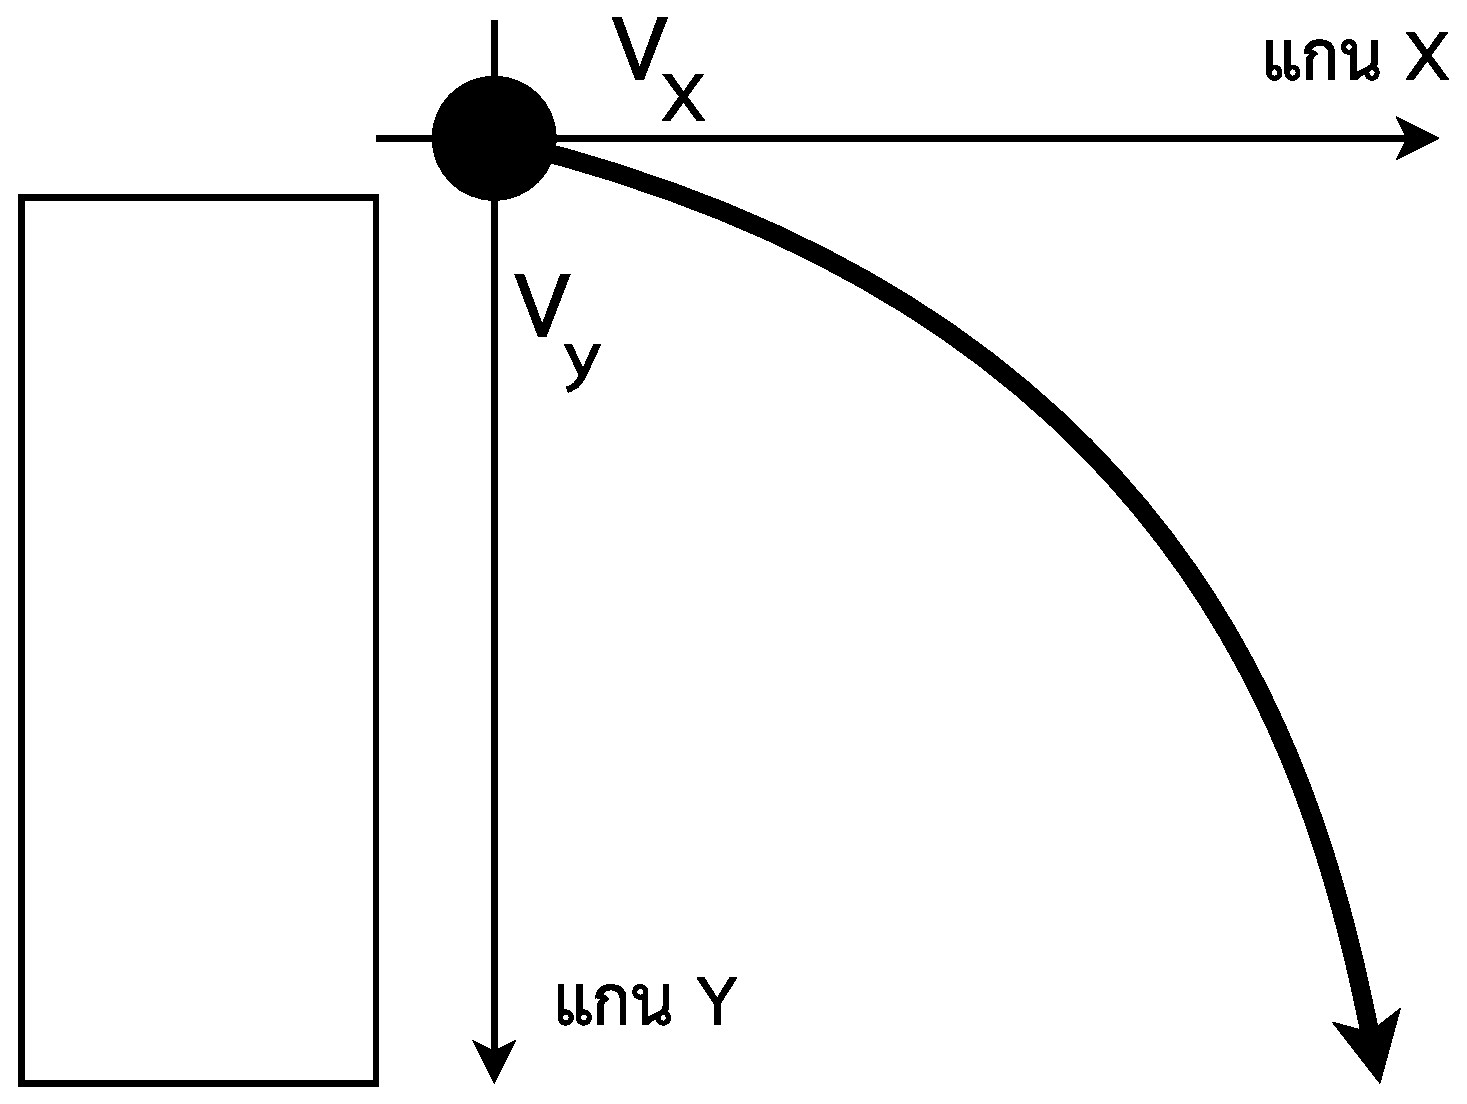
\includegraphics[width=0.4\textwidth]{content-8.eps}
  \end{center}
  \vspace{-20pt}
  \vspace{-10pt}
\end{wrapfigure}
\textbf{การเคลื่อนที่แบบโพรเจกไทล์}  คือ การเคลื่อนที่ในแนวโค้งรูปพาราโบลา  เกิดจากการเคลื่อนที่หลายมิติผสมกัน  ตัวอย่างเช่นหากเราขว้างวัตถุออกไปในแนวระดับจากดาดฟ้าตึกแห่งหนึ่ง  เราจะพบว่าวัตถุจะมีความพยายามที่จะเคลื่อนที่ไปในแนวระดับ (แกน X) ตามแรงที่เราขว้าง  พร้อมกันนั้นวัตถุจะถูกแรงโน้มถ่วงของโลก  ดึงให้เคลื่อนที่ตกลงมาในแนวดิ่ง (แกน Y) ด้วย    และเนื่องจากการเคลื่อนที่ทั้งสองแนวนี้เกิดในเวลาเดียวกัน      จึงเกิดการผสมผสานกันกลายเป็นการเคลื่อนที่แบบเส้นโค้งพาราโบลาพุ่งออกมาระหว่างกลางแนวระดับ (แกน X)  และแนวดิ่ง (แกน Y) ดังรูป  การเคลื่อนที่ในวิถีโค้งแบบนี้เรียกว่าเป็น \textbf{การเคลื่อนที่แบบโพรเจกไทล์}
